% Copyright 2004 by Till Tantau <tantau@users.sourceforge.net>.
%
% In principle, this file can be redistributed and/or modified under
% the terms of the GNU Public License, version 2.
%
% However, this file is supposed to be a template to be modified
% for your own needs. For this reason, if you use this file as a
% template and not specifically distribute it as part of a another
% package/program, I grant the extra permission to freely copy and
% modify this file as you see fit and even to delete this copyright
% notice. 

\documentclass[aspectratio=169]{beamer}
\usepackage{graphicx}
\usepackage{listings}
 
% There are many different themes available for Beamer. A comprehensive
% list with examples is given here:
% http://deic.uab.es/~iblanes/beamer_gallery/index_by_theme.html
% You can uncomment the themes below if you would like to use a different
% one:

%\usetheme{Malmoe}
%\usetheme{Marburg}
%\usetheme{Montpellier}
%\usetheme{PaloAlto}
%\usetheme{Pittsburgh}
%\usetheme{Rochester}
%\usetheme{Singapore}
%\usetheme{Szeged}
%\usetheme{Warsaw}
%\usetheme{AnnArbor}
%\usetheme{Antibes}
%\usetheme{Bergen}
%\usetheme{Berkeley}
%\usetheme{Berlin}
%\usetheme{Boadilla}
%\usetheme{boxes}
%\usetheme{CambridgeUS}
%\usetheme{Copenhagen}
%\usetheme{Darmstadt}
%\usetheme{default}
%\usetheme{Frankfurt}
%\usetheme{Goettingen}
%\usetheme{Hannover}
%\usetheme{Ilmenau}
%\usetheme{JuanLesPins}
%\usetheme{Luebeck}
\usetheme{Madrid}
 
\setbeamertemplate{footline}
 {
 	\leavevmode%
 	\hbox{%
 		%Author names
 		\begin{beamercolorbox}[wd=.7\paperwidth,ht=2.25ex,dp=1ex,center]{author in head/foot}%
 		\usebeamerfont{author in head/foot}\insertshortauthor
 		\end{beamercolorbox}%
 		
 		\begin{beamercolorbox}[wd=.2\paperwidth,ht=2.25ex,dp=1ex,center]{title in head/foot}%
 			\usebeamerfont{title in head/foot}\insertshorttitle
 		\end{beamercolorbox}%
	 
 		\begin{beamercolorbox}[wd=.1\paperwidth,ht=2.25ex,dp=1ex,center]{date in head/foot}%
 			\usebeamerfont{title in head/foot} \insertframenumber{} / \inserttotalframenumber
 		\end{beamercolorbox}}%
 		\vskip0pt%
 		}
\setbeamertemplate{navigation symbols}{}

\title{Game AI: Project 1}

% A subtitle is optional and this may be deleted
\subtitle{Simple-strategies for turn-based games}

\author{Mariia Rybalka \and Elchin Valiyev \and Abbas Khan \and Maxim Radomskyi \and Maxim Maltsev}
% - Give the names in the same order as the appear in the paper.
% - Use the \inst{?} command only if the authors have different
%   affiliation.

%\institute[Universities of Bonn] % (optional, but mostly needed)
%{
%  \inst{1}%
%  Department of Computer Science\\
%  University of Somewhere
%  \and
%  \inst{2}%
%  Department of Theoretical Philosophy\\
%  University of Elsewhere}
% - Use the \inst command only if there are several affiliations.
% - Keep it simple, no one is interested in your street address.

\date{Colloqium, 2016}
% - Either use conference name or its abbreviation.
% - Not really informative to the audience, more for people (including
%   yourself) who are reading the slides online

\subject{Theoretical Computer Science}
% This is only inserted into the PDF information catalog. Can be left
% out. 

% If you have a file called "university-logo-filename.xxx", where xxx
% is a graphic format that can be processed by latex or pdflatex,
% resp., then you can add a logo as follows:

% \pgfdeclareimage[height=0.5cm]{university-logo}{university-logo-filename}
% \logo{\pgfuseimage{university-logo}}

% Delete this, if you do not want the table of contents to pop up at
% the beginning of each subsection:
\AtBeginSubsection[]
{
  \begin{frame}<beamer>{Outline:}
    \tableofcontents[currentsection,currentsubsection]
  \end{frame}
}

% Let's get started
\begin{document}

\defverbatim[colored]\lstMinMax{
	\begin{lstlisting}[language=Python,basicstyle=\tiny,keywordstyle=\color{red}]
def minmax(board, player, max_depth, current_depth):
	# Check if we're done recursing
	if board.game_is_over() or current_depth == max_depth:
		return board.evaluate(player), None

	best_move = None
	if board.current_player() == player:
		best_score = -INFINITY
	else:
		best_score = INFINITY

	# Go through each move
	for move in board.get_moves():
		new_board = board.makeove(move)

		# Recurse
		current_score, current_move = minmax(new_board, player, max_depth, current_depth + 1)

		# Update the best score
		if board.current_player() == player:
			if current_score > best_score:
				best_score = current_score
				best_move = move
			else:
				if current_score < best_score:
					best_score = current_score
					best_move = move

	# Return the score and the best move
	return best_score, best_move
	
	\end{lstlisting}
}





\begin{frame}
  \titlepage
\end{frame}

\begin{frame}{Outline }
  \tableofcontents
  % You might wish to add the option [pausesections]
\end{frame}

% Section and subsections will appear in the presentation overview
% and table of contents.
\section{Simple strategies for tic tac toe}

\subsection{Probabilistic strategy}

\begin{frame}{Probabilistic strategy slide 1}{Optional Subtitle}
	content ... 
\end{frame}

\begin{frame}{Performance}
	
\end{frame}

\subsection{Heuristic strategy}

% You can reveal the parts of a slide one at a time
% with the \pause command:
\begin{frame}{Evaluating the quality of a potential move}

How to pick next move from possible ones? \\
We need to see difference! 
\begin{figure}
	\includegraphics[scale = 0.5]{not_known.png}	
\end{figure}
\end{frame}

\begin{frame}{Heuristic / Evaluation function}
Provides an estimate of the utility of a game state that is
not a terminal state
\begin{block}{Simple evaluation function for Tic-Tac-Toe (from slides)}
\textbf{Eval(n, p)} = (number of lines where \textbf{p} can win) $-$ (number of lines where \textbf{-p} can win)
\end{block}
\only<1>{
\begin{figure}
	\includegraphics[scale = 0.5]{not_known.png}
\end{figure}}

\only<2->{\begin{figure}
		\includegraphics[scale = 0.5]{eval_1b.png}
	\end{figure}}
\pause
 Obviously, current function is not a good one! We can do better!
\end{frame}



\begin{frame}{Heuristic / Evaluation function (cont.)}

\begin{block}{A Better Evaluation Function   (Russell \& Norvig, Artificial Intelligence)}
Eval(n) = 3 * X2 + X1 – (3 * O2 + O1) \\

\begin{itemize}
 \item X2 is the number of lines with 2 X’s and a blank
 \item X1 is the number of lines with 1 X and 2 blanks
 \item O2 is the number of lines with 2 O’s and a blank
 \item O1 is the number of lines with 1 O and 2 blanks 
\end{itemize}

\end{block}
\only<1>{\begin{figure}
	\includegraphics[scale = 0.5]{not_known.png}
\end{figure}}

\only<2->{\begin{figure}
 \includegraphics[scale = 0.5]{eval_2a.png}
\end{figure}}
\end{frame}

\begin{frame}{Minmax algorithm}
	
\lstMinMax
\end{frame}

\begin{frame}{Performance}
	 \begin{columns}
	 	\begin{column}{0.5\textwidth}
	 		\centering
	 		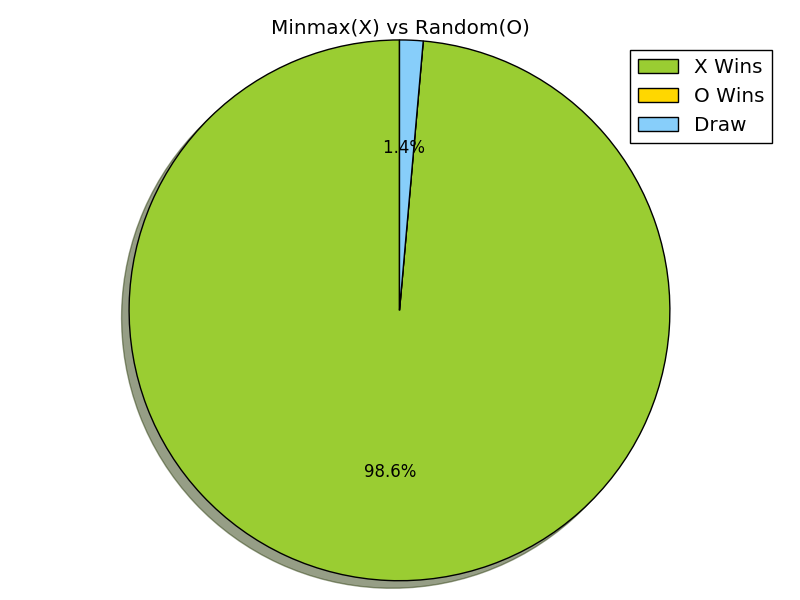
\includegraphics[scale =0.35]{minmax_random.png}
	 	\end{column}
	 	\begin{column}{0.5\textwidth}
	 		\centering
	 		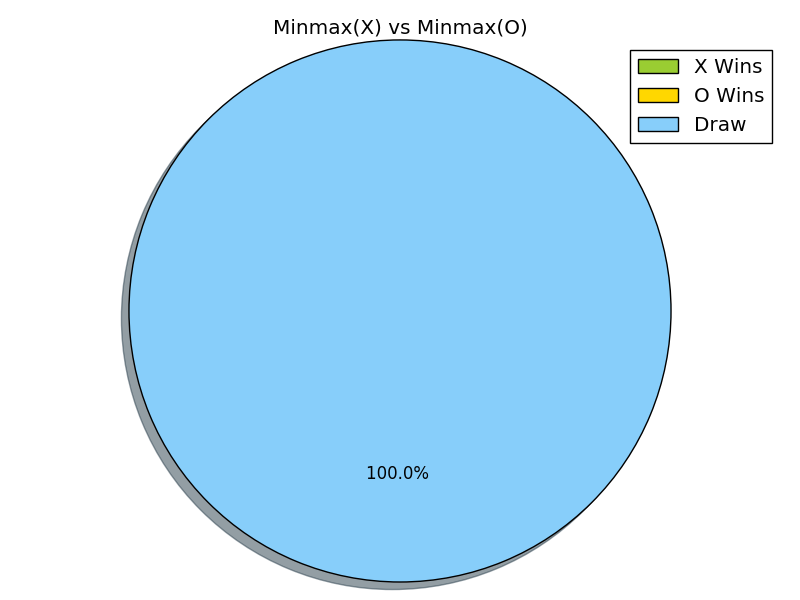
\includegraphics[scale =0.35]{minmax_minmax.png}
	 	\end{column}
	 \end{columns}
\end{frame}

\section{Connect 4}

\subsection{Another Subsection}

\begin{frame}{Connect 4 Slide 1}
	content ...
\end{frame}

\begin{frame}{Connect 4 Slide 2}
	content...
\end{frame}



% Placing a * after \section means it will not show in the
% outline or table of contents.
\section*{Summary}

\begin{frame}{Do we need Summary ?}
	
\end{frame}

\begin{frame}{That's All Folks!}
	\begin{center}
     {\huge	Thank you for attention! }
	\end{center}
	
\end{frame}

\end{document}


